% 0 - O
% 1 - I
% 2 - L
% 3  - E
% 4 - A
% 5 - S
% 6 - C
% 7 - T
% 8 - B 13
% 9 - G
\graphicspath{{images/}}
\newcommand{\GVLO}{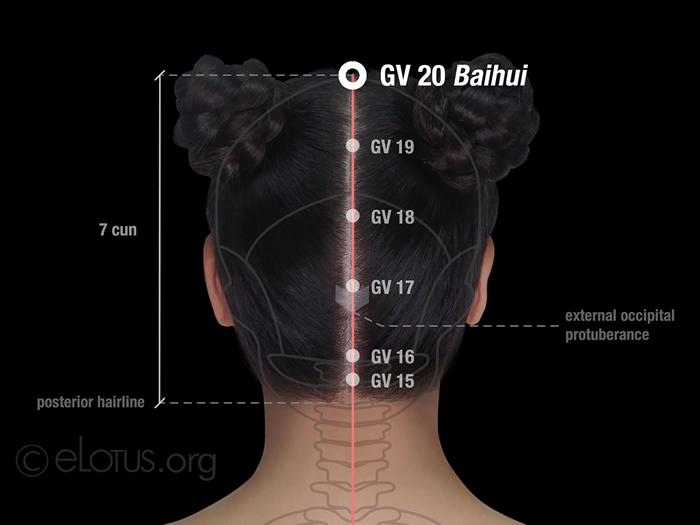
\includegraphics[width=\linewidth]{GV20_0.png}}
\newcommand{\GBLO}{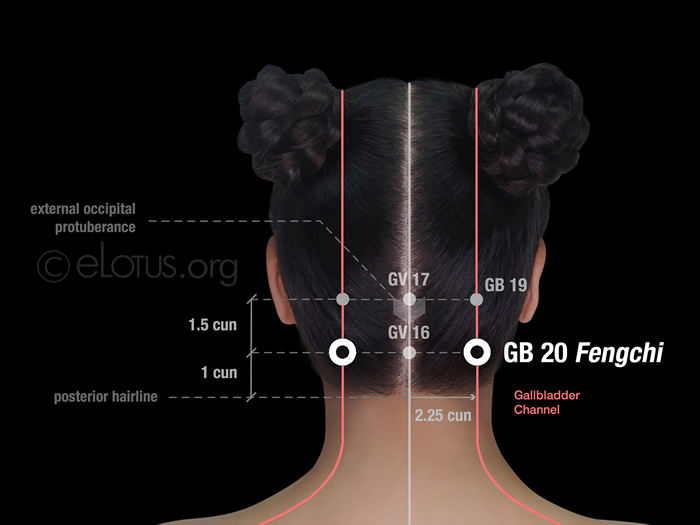
\includegraphics[width=\linewidth]{GB20.png}}
\newcommand{\STB}{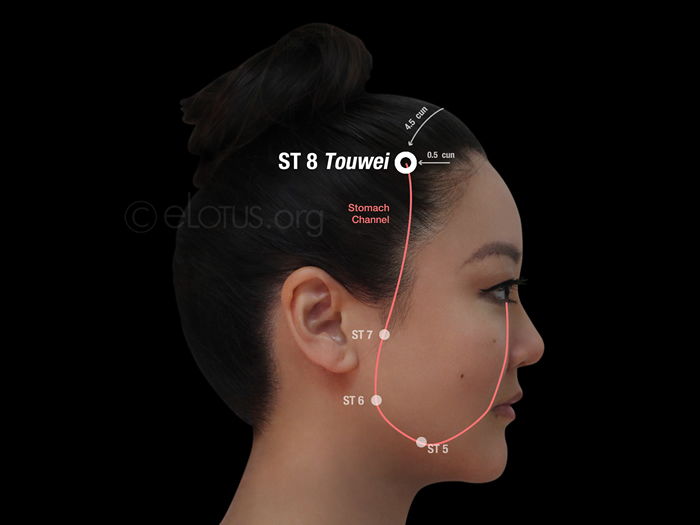
\includegraphics[width=\linewidth]{ST8.png}}
\newcommand{\GBB}{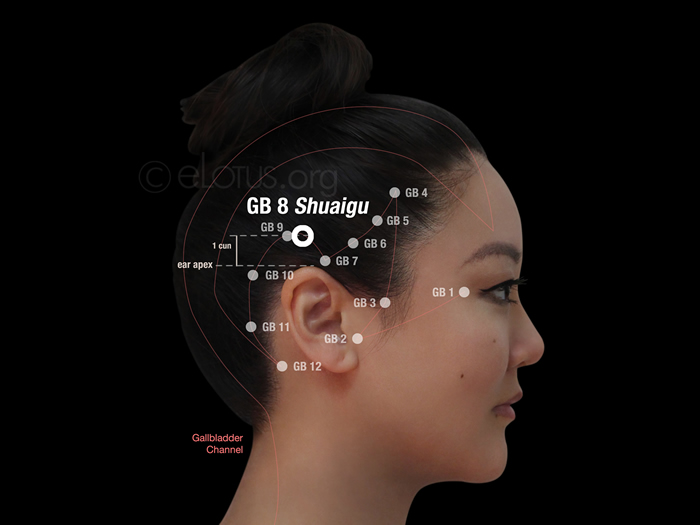
\includegraphics[width=\linewidth]{GB8.png}}
\newcommand{\ExHNS}{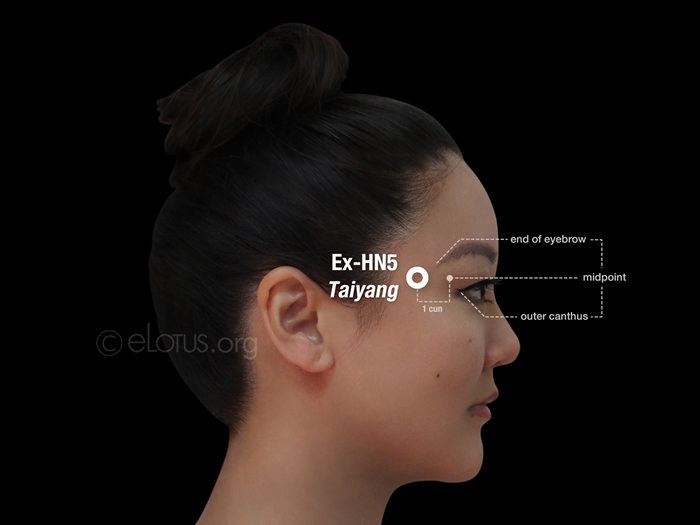
\includegraphics[width=\linewidth]{Ex-HN5.png}}
\newcommand{\AnDuong}{Ex-HN3.png}
\newcommand{\ExHNE}{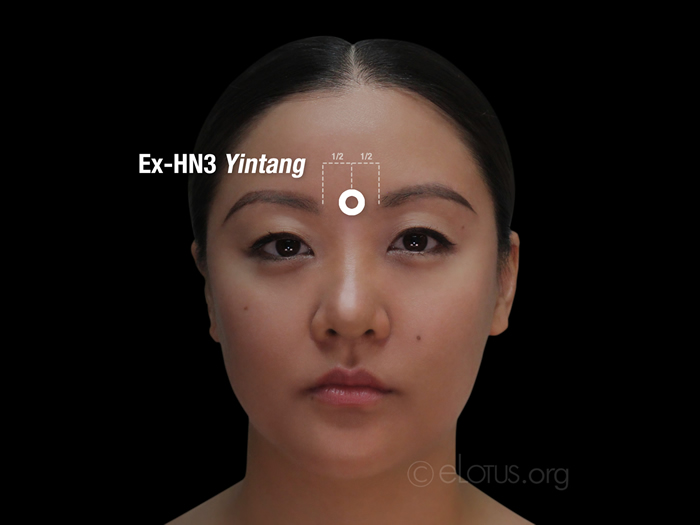
\includegraphics[width=\linewidth]{Ex-HN3.png}}
\newcommand{\BLIO}{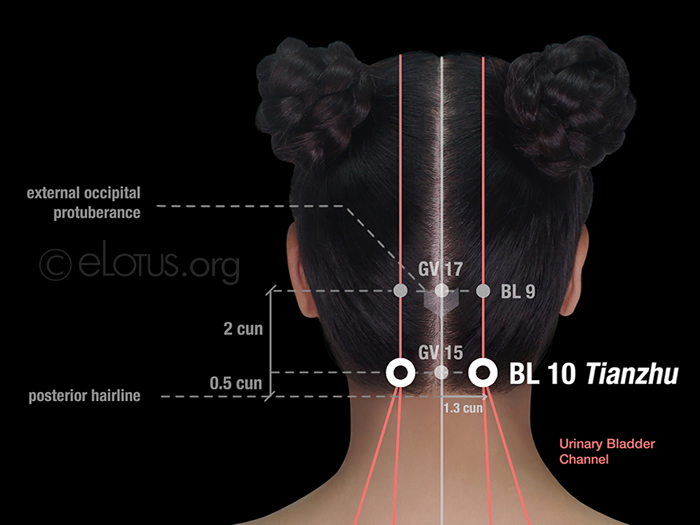
\includegraphics[width=\linewidth]{BL10.png}}
\newcommand{\GBLI}{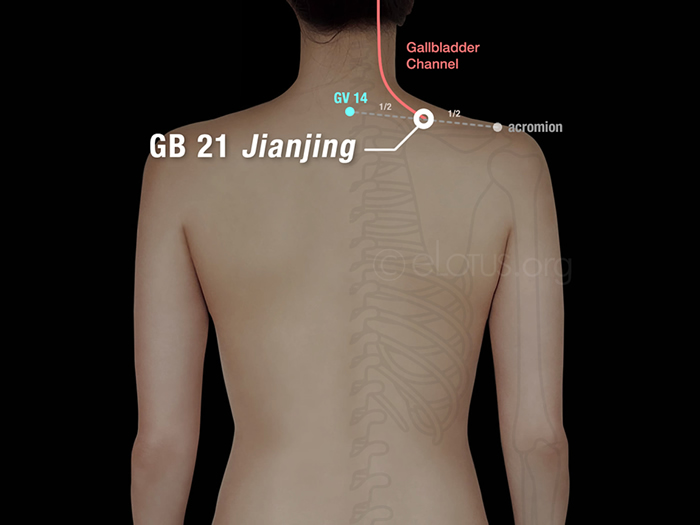
\includegraphics[width=\linewidth]{GB21.png}}
\newcommand{\LUI}{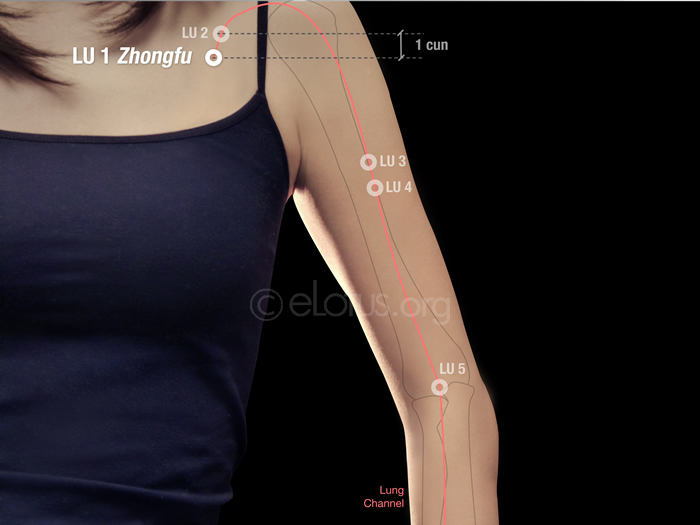
\includegraphics[width=\linewidth]{LU1.png}}
\newcommand{\BLIL}{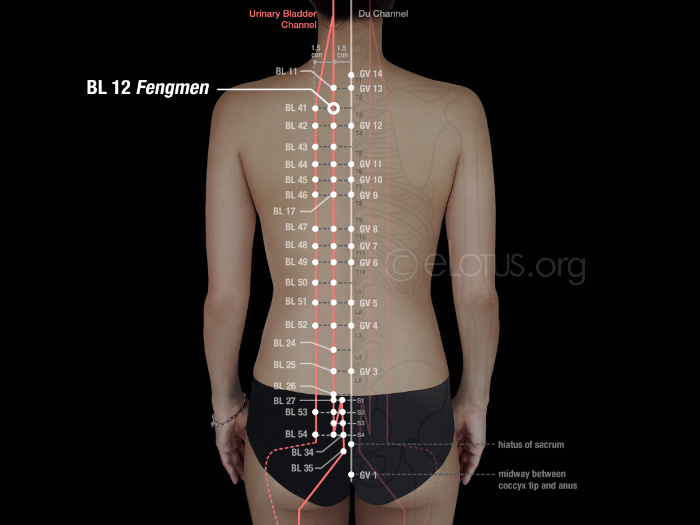
\includegraphics[width=\linewidth]{BL12.png}}
\newcommand{\LIIS}{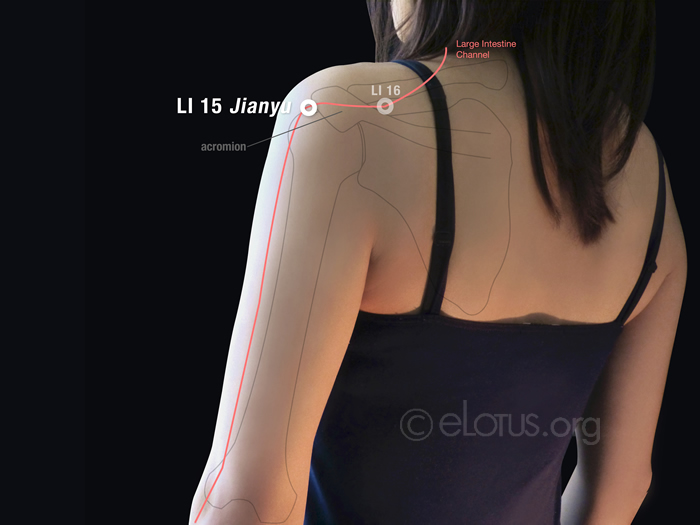
\includegraphics[width=\linewidth]{LI15b.png}}
\newcommand{\LIIC}{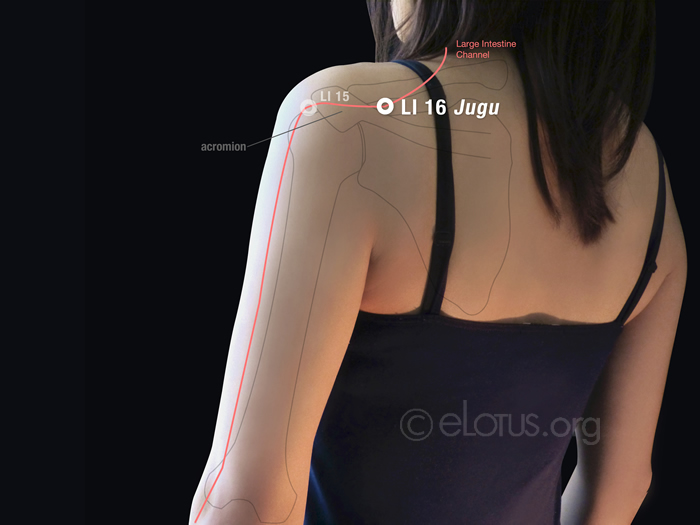
\includegraphics[width=\linewidth]{LI_16b.png}}
\newcommand{\SIIO}{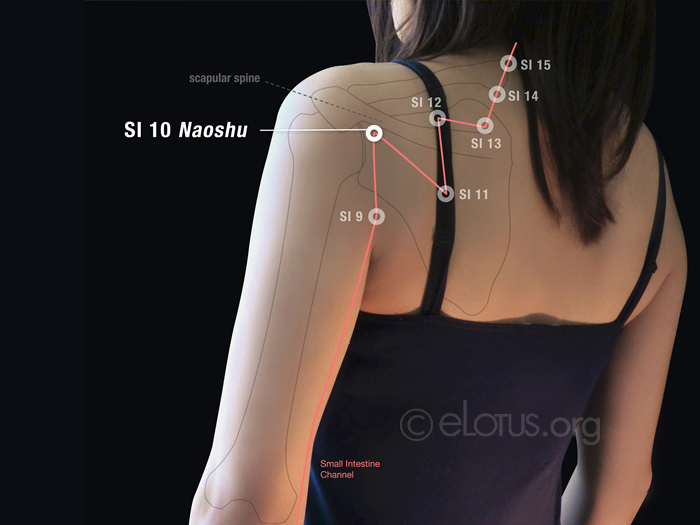
\includegraphics[width=\linewidth]{SI10.png}}
\newcommand{\SIII}{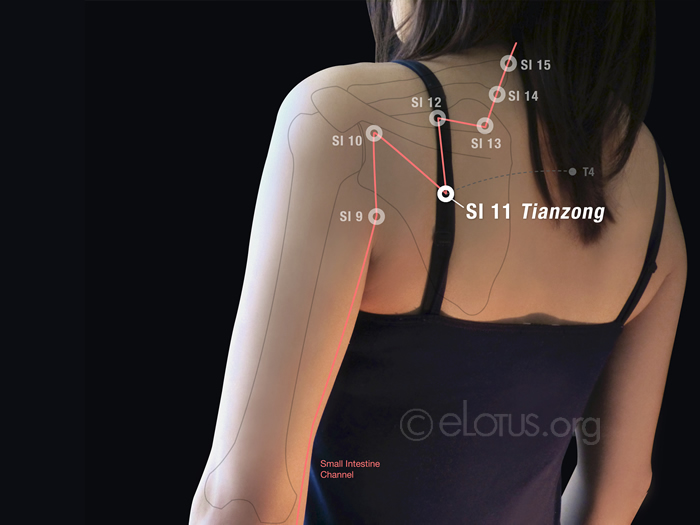
\includegraphics[width=\linewidth]{SI_11.png}}
\newcommand{\LIIA}{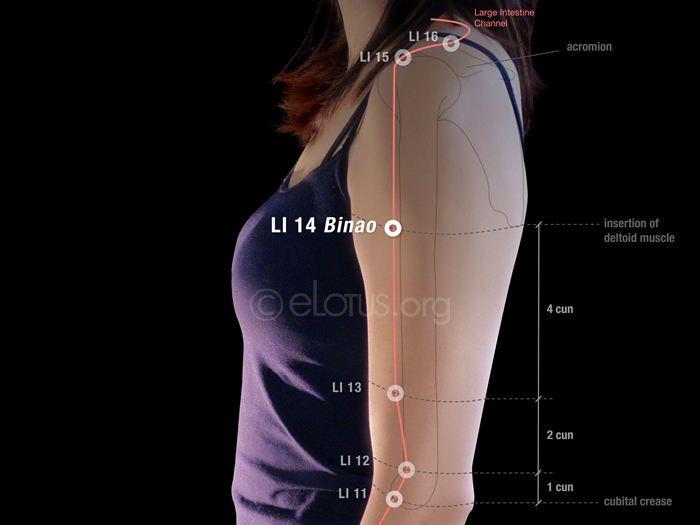
\includegraphics[width=\linewidth]{LI_14.png}}
\newcommand{\EXBL}{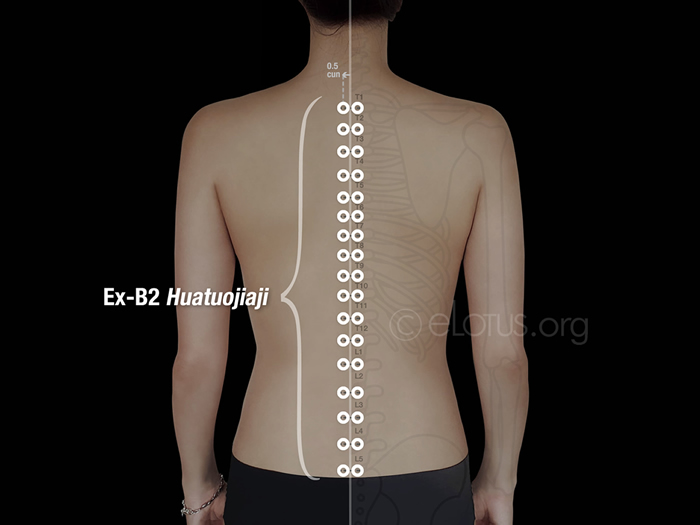
\includegraphics[width=\linewidth]{Ex_B2.png}}
\newcommand{\BLLE}{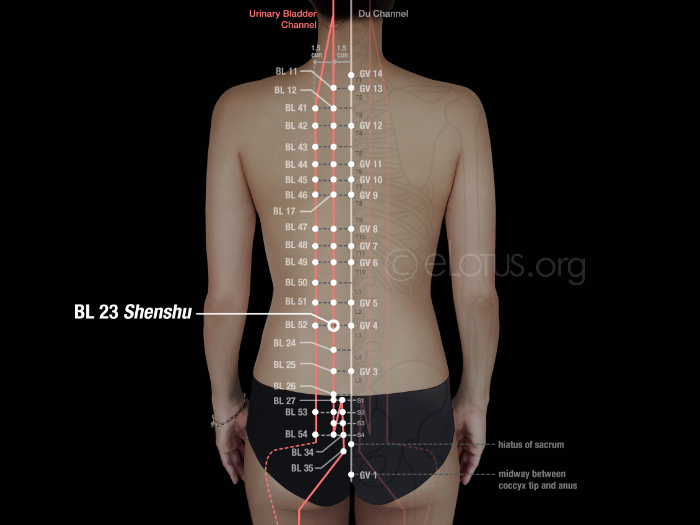
\includegraphics[width=\linewidth]{BL_23.png}}
\newcommand{\BLIT}{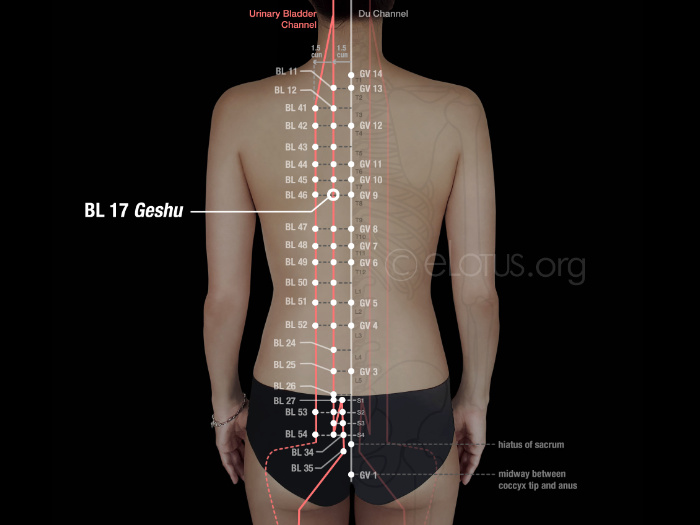
\includegraphics[width=\linewidth]{BL_17.png}}
\newcommand{\BLLS}{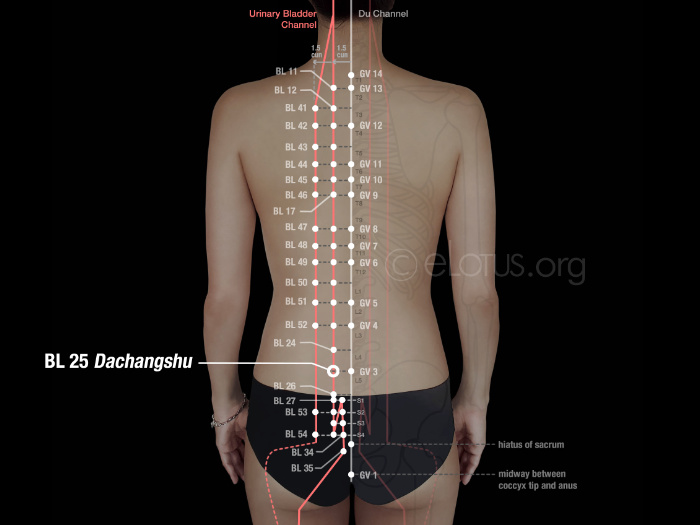
\includegraphics[width=\linewidth]{BL_25.png}}
\newcommand{\GBEO}{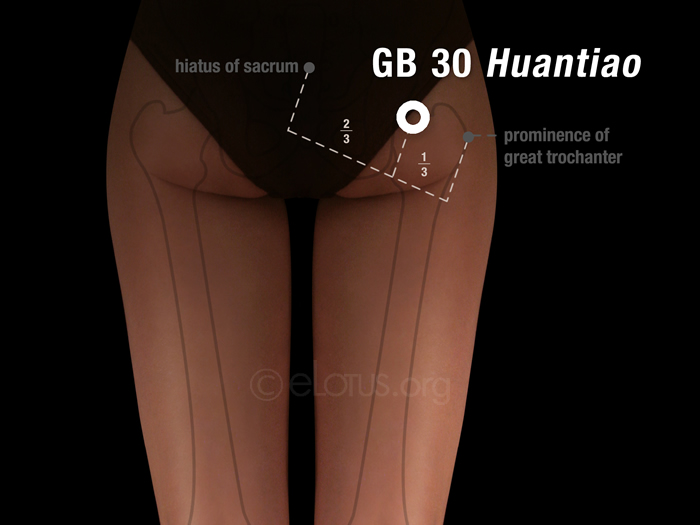
\includegraphics[width=\linewidth]{GB_30.png}}
\newcommand{\BLEC}{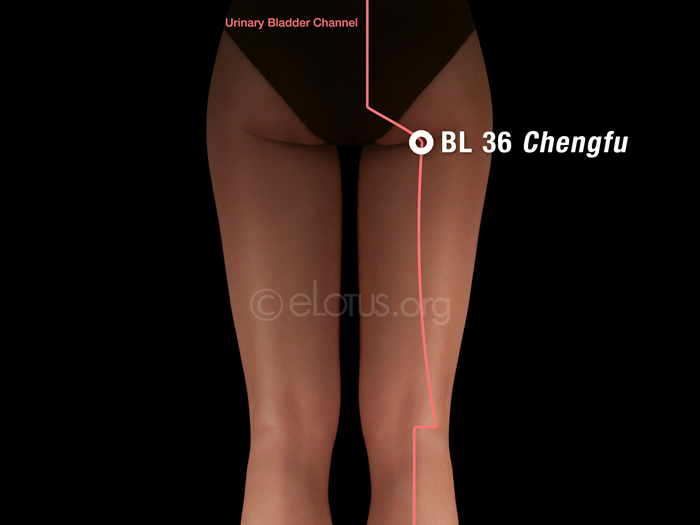
\includegraphics[width=\linewidth]{BL_36.png}}
\newcommand{\BLAO}{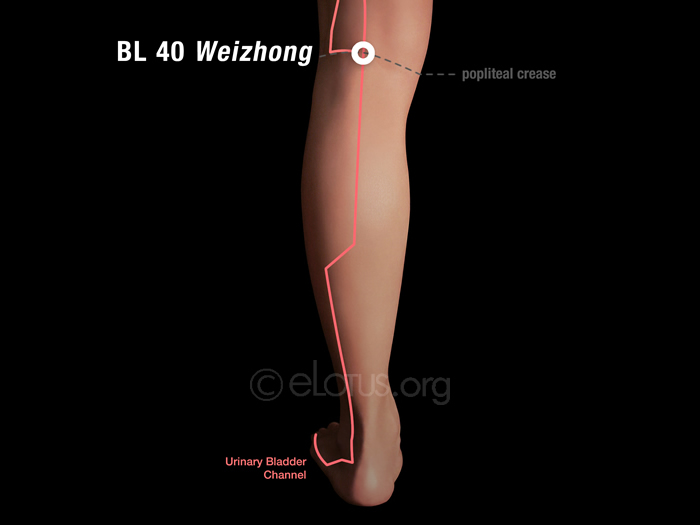
\includegraphics[width=\linewidth]{BL_40.png}}
\newcommand{\BLST}{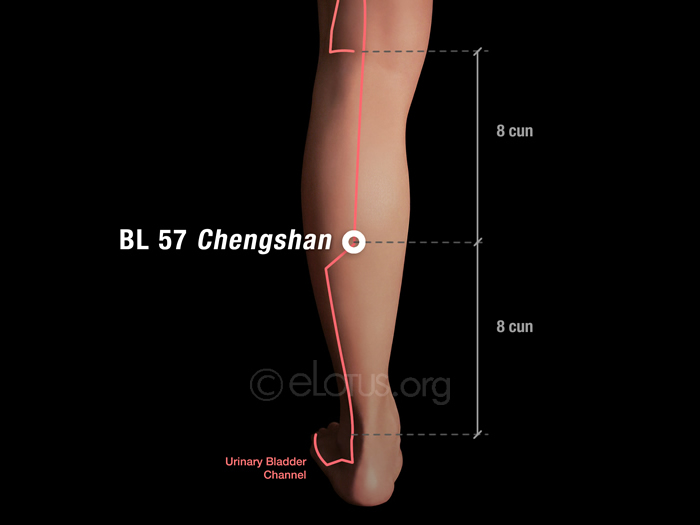
\includegraphics[width=\linewidth]{BL_57.png}}
\newcommand{\BLCO}{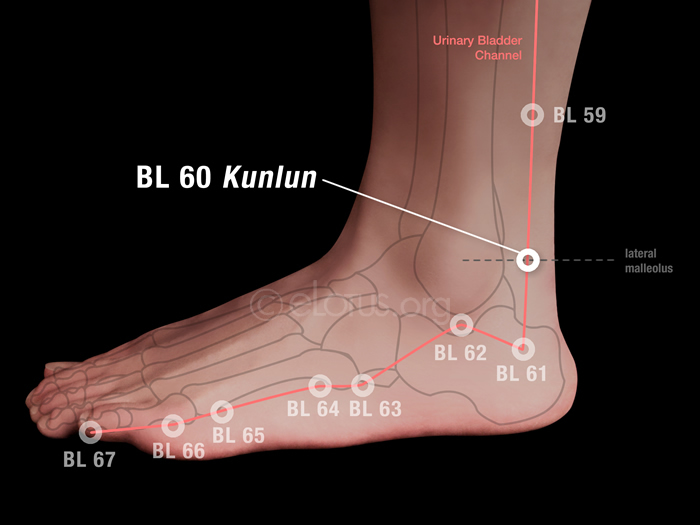
\includegraphics[width=\linewidth]{BL_60.png}}
\newcommand{\GBEI}{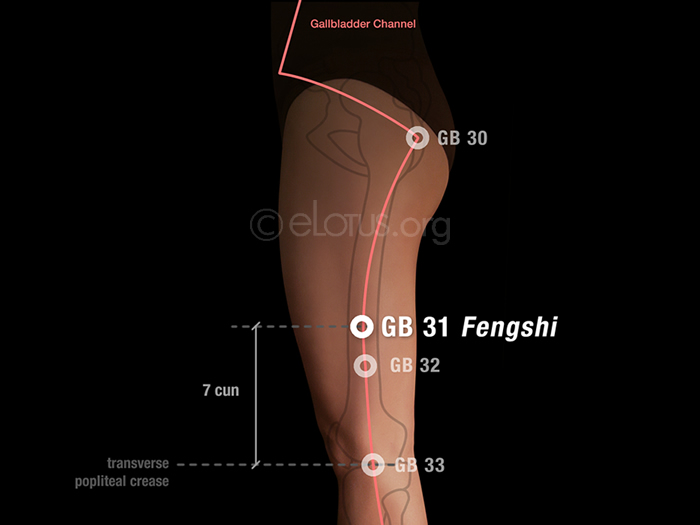
\includegraphics[width=\linewidth]{GB_31.png}}
\newcommand{\GBEA}{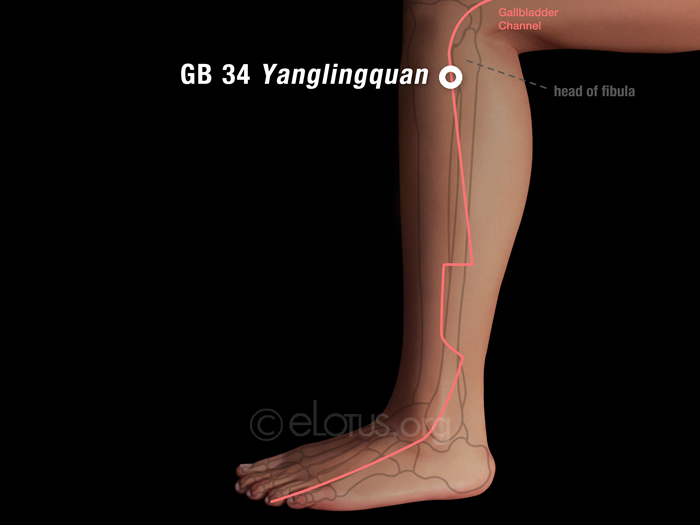
\includegraphics[width=\linewidth]{GB_34.png}}
\newcommand{\BLI}{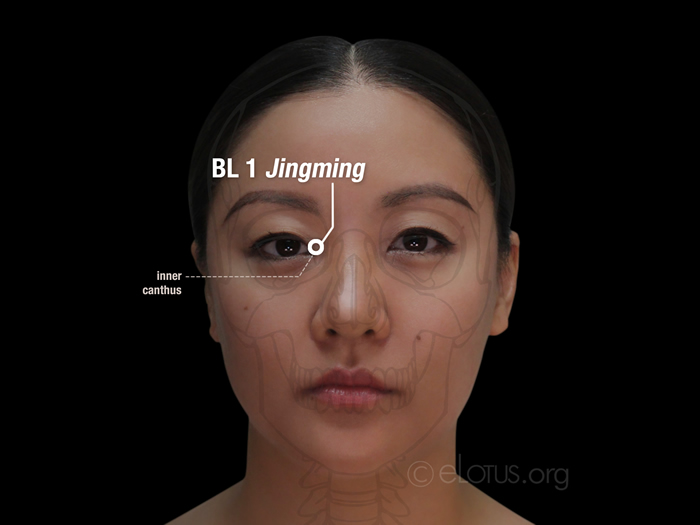
\includegraphics[width=\linewidth]{BL_1.png}}
\newcommand{\BLL}{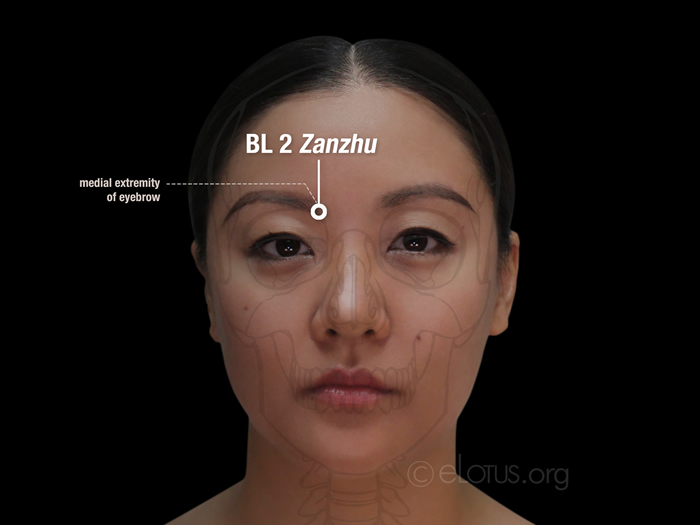
\includegraphics[width=\linewidth]{BL_2.png}}
\newcommand{\LILO}{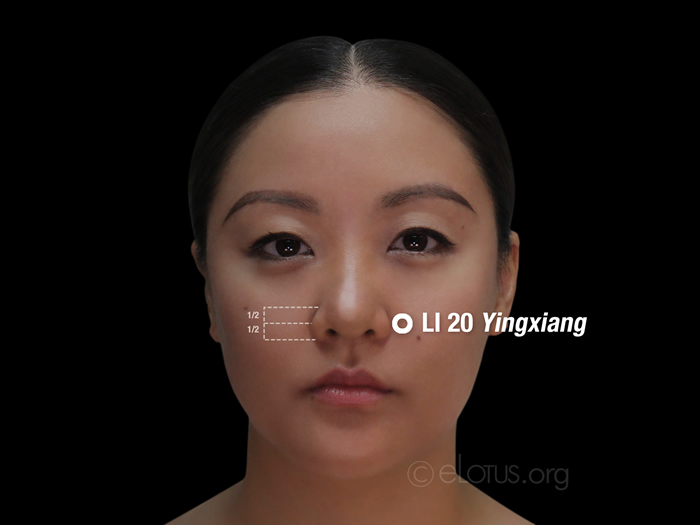
\includegraphics[width=\linewidth]{LI_20.png}}
\newcommand{\STA}{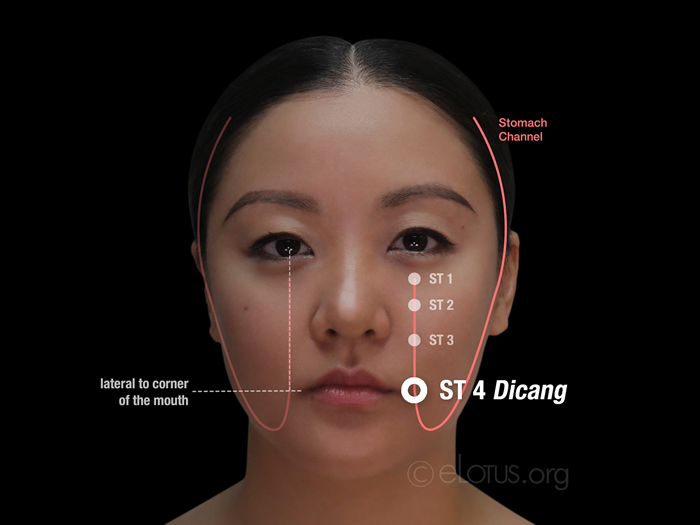
\includegraphics[width=\linewidth]{ST_4.png}}
\newcommand{\GVLC}{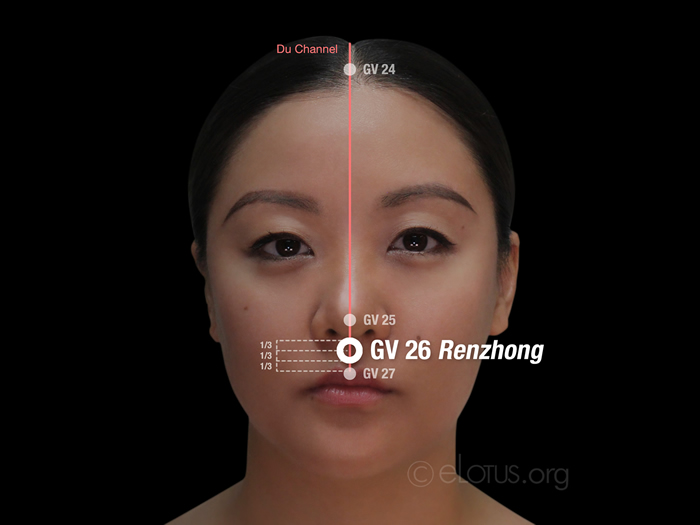
\includegraphics[width=\linewidth]{GV_26.png}}
\newcommand{\CVLA}{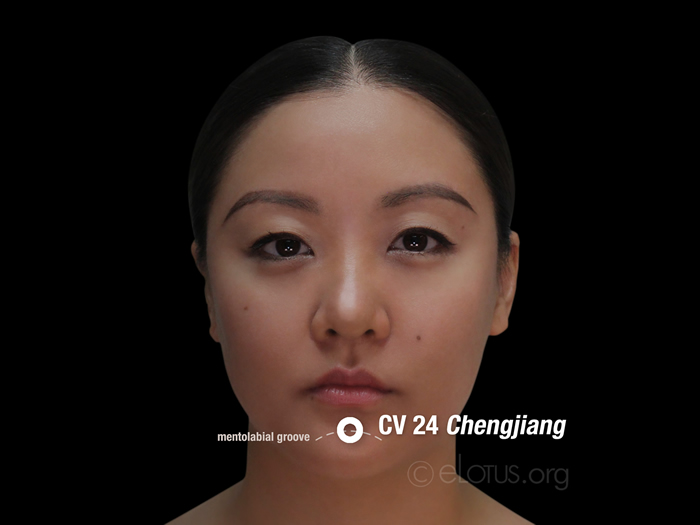
\includegraphics[width=\linewidth]{CV_24.png}}
\newcommand{\EXHNA}{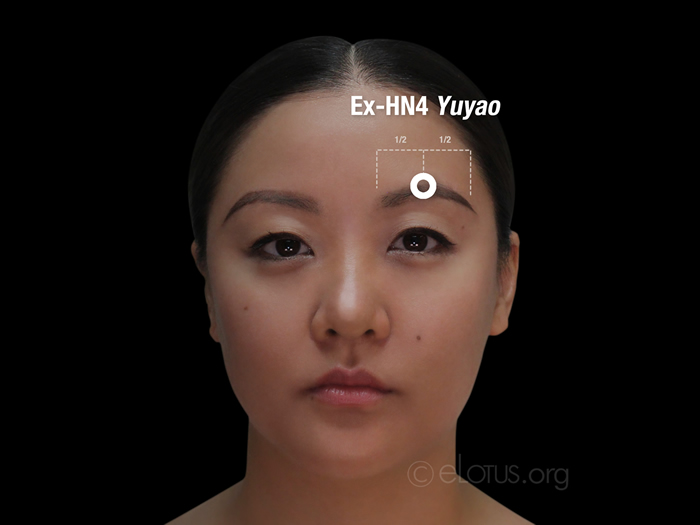
\includegraphics[width=\linewidth]{Ex_HN4.png}}
\newcommand{\LIA}{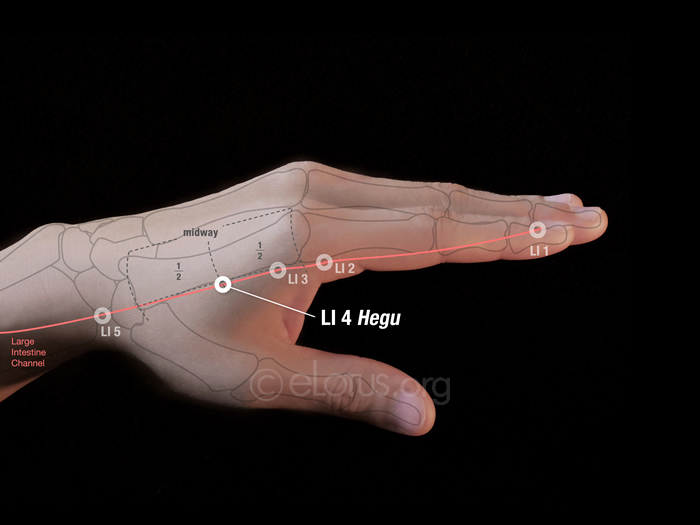
\includegraphics[width=\linewidth]{LI_4.png}}
\newcommand{\THA}{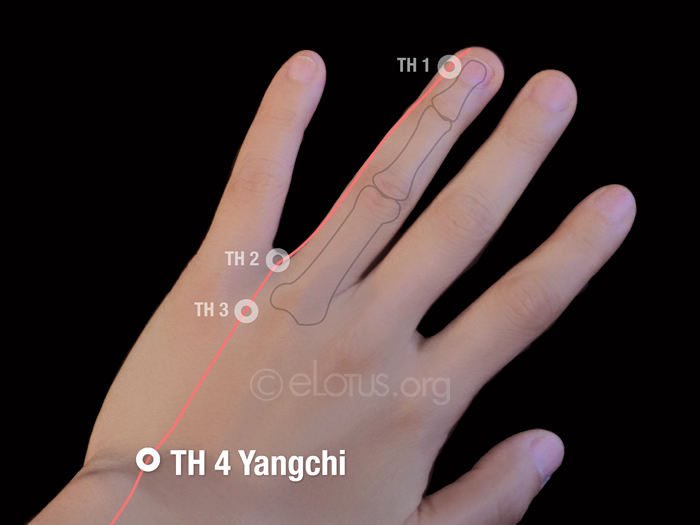
\includegraphics[width=\linewidth]{TH_4.png}}
\newcommand{\PCB}{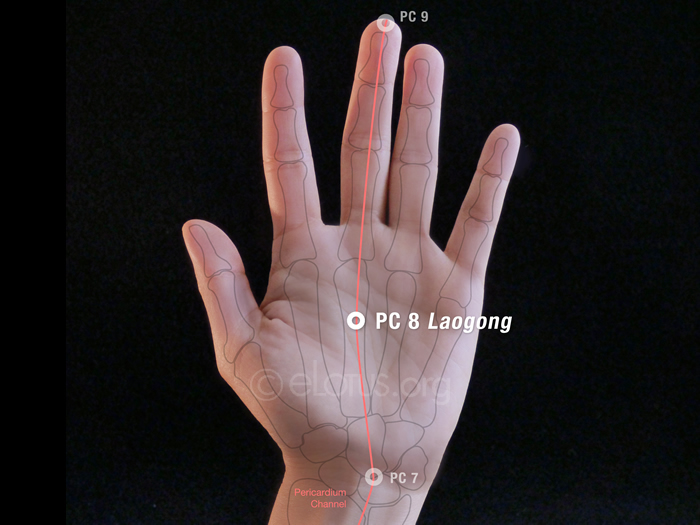
\includegraphics[width=\linewidth]{PC_8.jpg}}
\LetLtxMacro{\laogong}{\PCB}
\LetLtxMacro{\laocung}{\PCB}

\newcommand{\PCT}{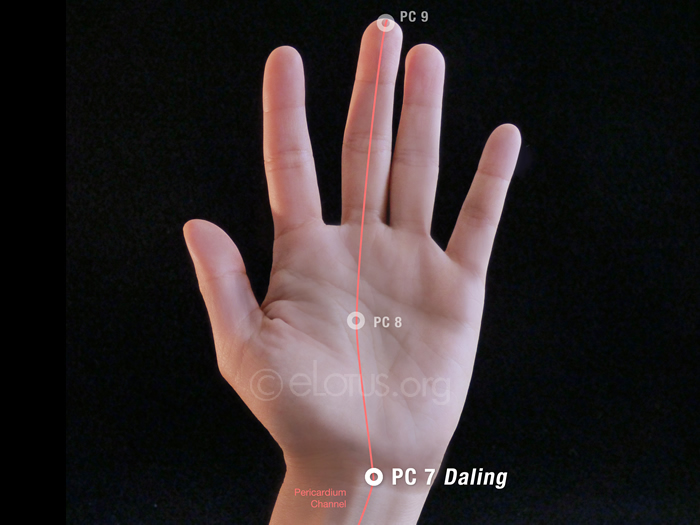
\includegraphics[width=\linewidth]{PC_7.jpg}}
\LetLtxMacro{\daling}{\PCT}
\LetLtxMacro{\dailang}{\PCT}

\newcommand{\LUIO}{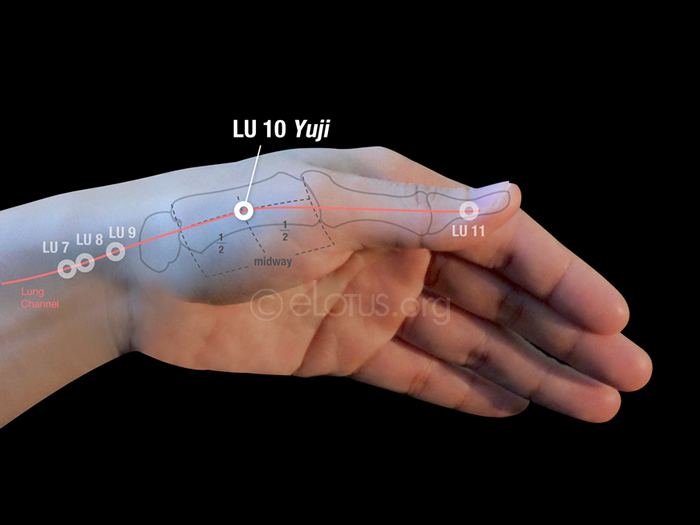
\includegraphics[width=\linewidth]{LU_10.jpg}}
\LetLtxMacro{\yuji}{\LUIO}
\LetLtxMacro{\ngute}{\LUIO}

\newcommand{\LUS}{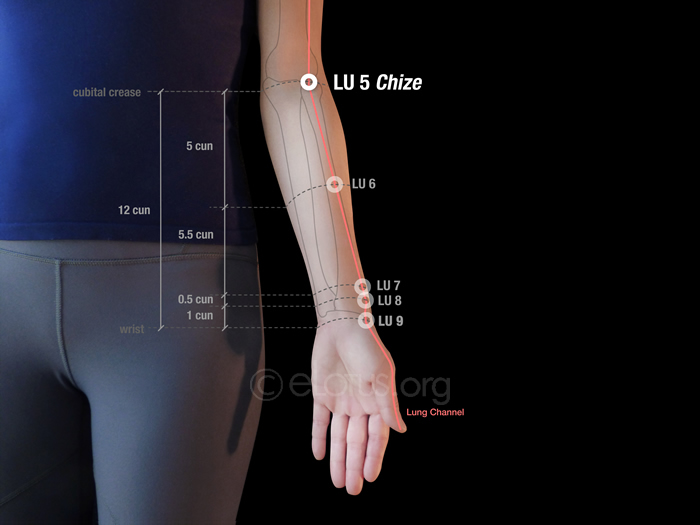
\includegraphics[width=\linewidth]{LU_5.jpg}}
\LetLtxMacro{\chize}{\LUS}
\LetLtxMacro{\xichtrach}{\LUS}

\newcommand{\LIIO}{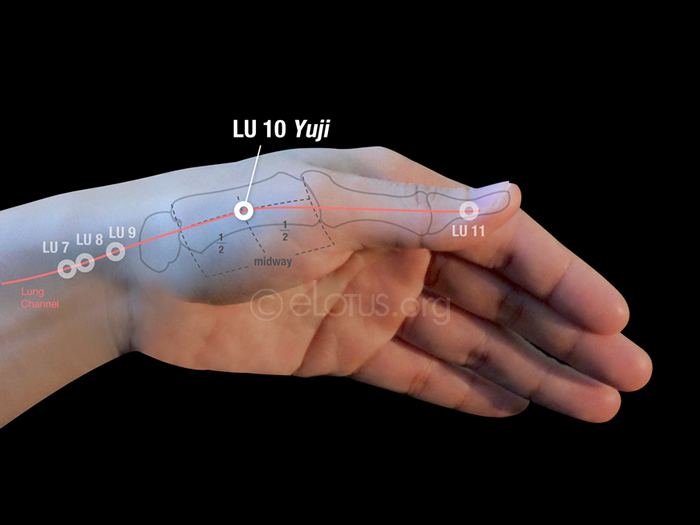
\includegraphics[width=\linewidth]{LU_10.jpg}}
\LetLtxMacro{\shousanli}{\LIIO}
\LetLtxMacro{\thutamly}{\LIIO}

\newcommand{\THS}{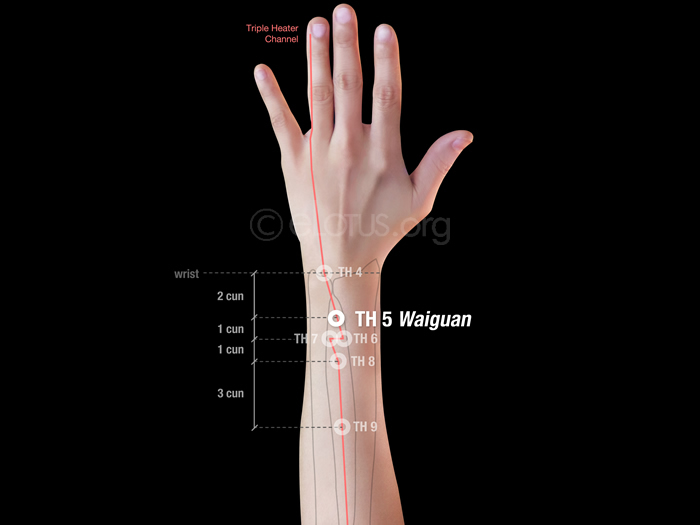
\includegraphics[width=\linewidth]{TH_5.jpg}}
\LetLtxMacro{\waiguan}{\THS}
\LetLtxMacro{\ngoaiquan}{\THS}

\newcommand{\LIII}{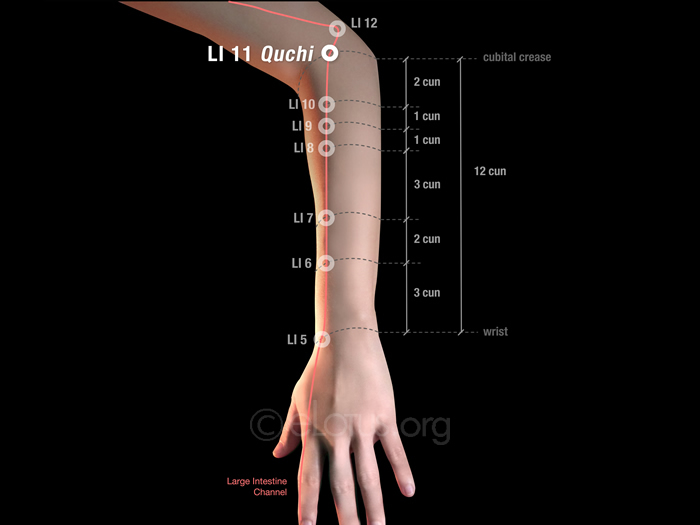
\includegraphics[width=\linewidth]{LI_11.png}}

\newcommand{\STC}{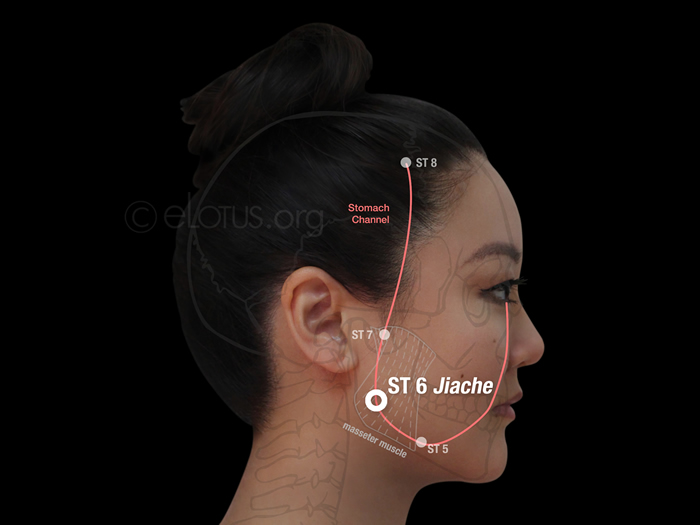
\includegraphics[width=\linewidth]{ST_6.png}}
\newcommand{\STT}{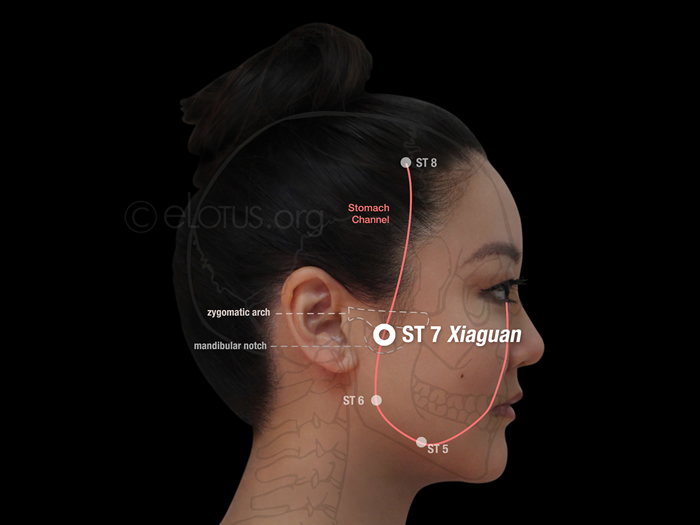
\includegraphics[width=\linewidth]{ST_7.png}}
\newcommand{\BLAE}{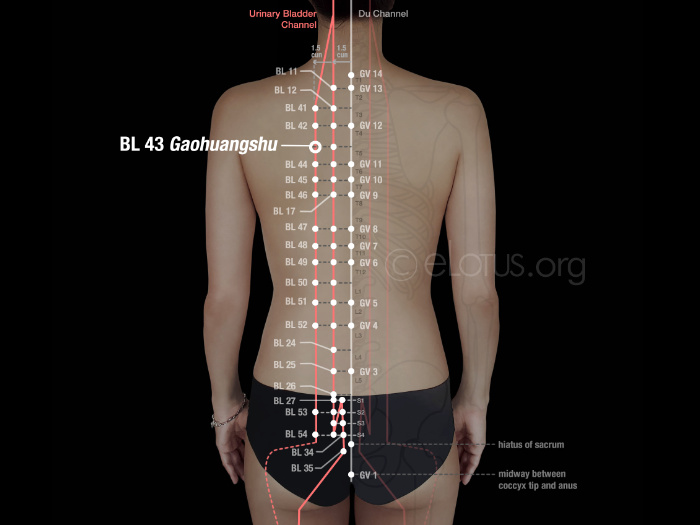
\includegraphics[width=\linewidth]{BL_43.png}}
\newcommand{\BLET}{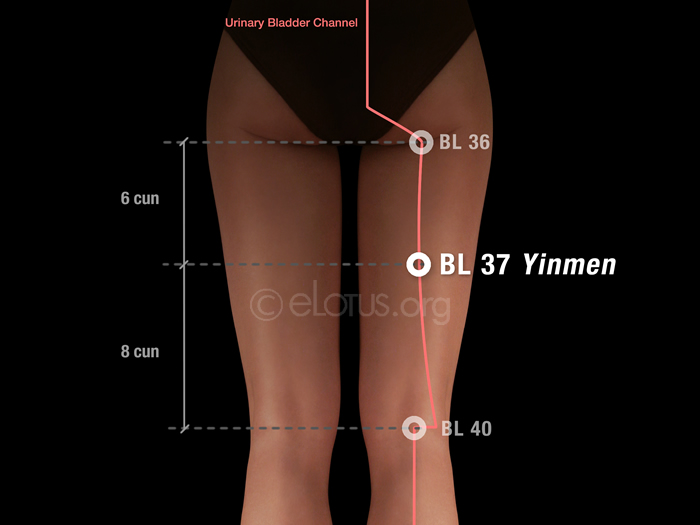
\includegraphics[width=\linewidth]{BL_37.png}}
\newcommand{\GBEG}{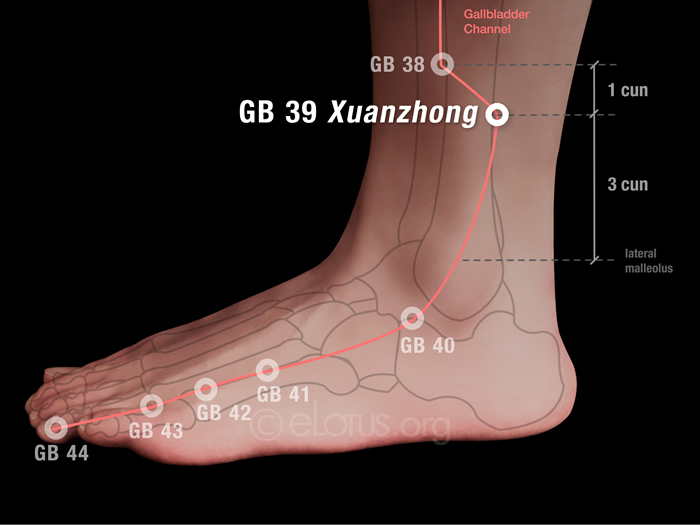
\includegraphics[width=\linewidth]{GB_39.png}}
\newcommand{\STAI}{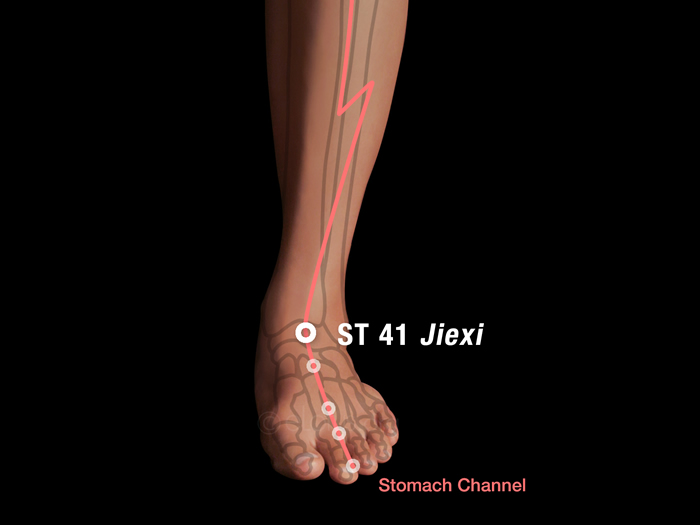
\includegraphics[width=\linewidth]{ST_41.png}}
\newcommand{\HTT}{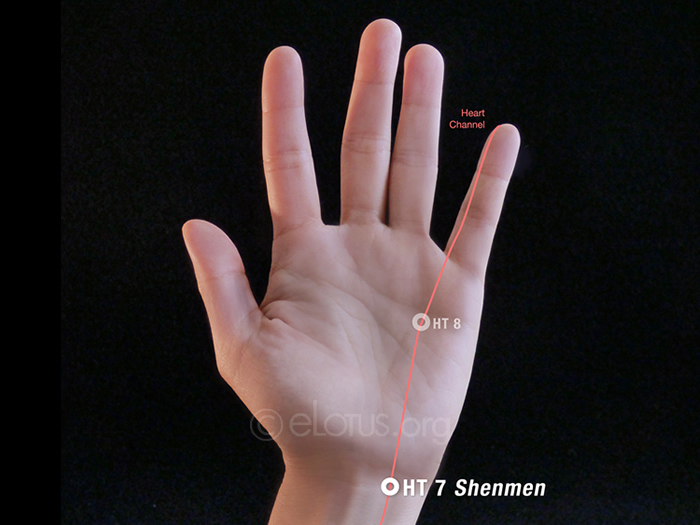
\includegraphics[width=\linewidth]{HT_7a.png}}
\newcommand{\KII}{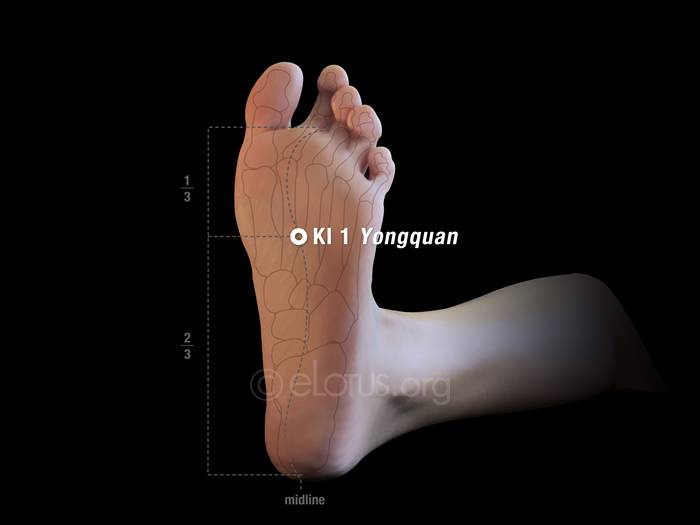
\includegraphics[width=\linewidth]{KI_1.png}}
\newcommand{\PCC}{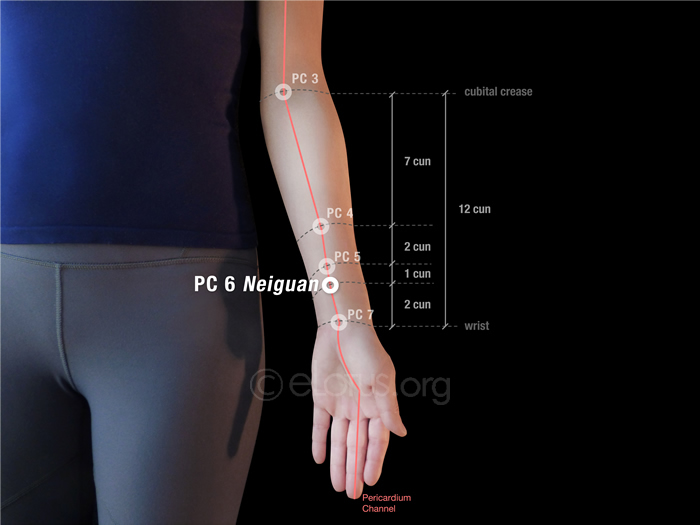
\includegraphics[width=\linewidth]{PC_6.png}}
\newcommand{\SPC}{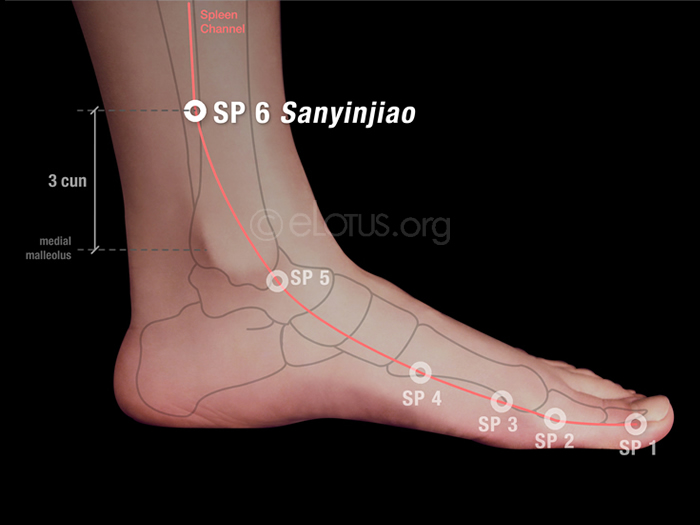
\includegraphics[width=\linewidth]{SP_6.png}}

\newcommand{\GBIA}{\includegraphics[width=\linewidth]{"GB 14.jpg"}}
\LetLtxMacro{\yangbai}{\GBIA}
\LetLtxMacro{\duongbach}{\GBIA}

\newcommand{\HNI}{\includegraphics[width=\linewidth]{"HN1.jpg"}}
\LetLtxMacro{\sishencong}{\HNI}
\LetLtxMacro{\tuthanthong}{\HNI}

\newcommand{\GBA}{\includegraphics[width=\linewidth]{"GB 4.jpg"}}
\LetLtxMacro{\hanyan}{\GBA}
\LetLtxMacro{\hamyen}{\GBA}

\newcommand{\GVIC}{\includegraphics[width=\linewidth]{"GV16.jpg"}}
\LetLtxMacro{\fengfu}{\GVIC}
\LetLtxMacro{\phongphu}{\GVIC}

\newcommand{\SIIT}{\includegraphics[width=\linewidth]{"SI 17.jpg"}}
\LetLtxMacro{\thiendung}{\SIIT}
\LetLtxMacro{\tianrong}{\SIIT}

\newcommand{\EXHNIS}{\includegraphics[width=\linewidth]{"Ex-HN15.jpg"}}
\LetLtxMacro{\bachlao}{\EXHNIS}
\LetLtxMacro{\jingbailao}{\EXHNIS}


\newcommand{\BLIE}{\includegraphics[width=\linewidth]{"Ex-HN15.jpg"}}
\LetLtxMacro{\phedu}{\BLIE}
\LetLtxMacro{\feishu}{\BLIE}


\newcommand{\BLIA}{\includegraphics[width=\linewidth]{"BL_14.jpg"}}
\LetLtxMacro{\quyetamdu}{\BLIA}
\LetLtxMacro{\jueyinshu}{\BLIA}


\newcommand{\BLIC}{\includegraphics[width=\linewidth]{"BL_16.jpg"}}
\LetLtxMacro{\docdu}{\BLIC}
\LetLtxMacro{\dushu}{\BLIC}

\newcommand{\SIG}{\includegraphics[width=\linewidth]{"SI_9.jpg"}}
\LetLtxMacro{\kientrinh}{\SIG}
\LetLtxMacro{\jianzhen}{\SIG}

\LetLtxMacro{\geshu}{\BLIT}

\newcommand{\BLIB}{\includegraphics[width=\linewidth]{"BL_18.jpg"}}
\LetLtxMacro{\candu}{\BLIB}
\LetLtxMacro{\canshu}{\BLIB}

\newcommand{\BLIG}{\includegraphics[width=\linewidth]{"BL_19.jpg"}}
\LetLtxMacro{\domdu}{\BLIG}

\newcommand{\BLLO}{\includegraphics[width=\linewidth]{"BL_20.jpg"}}
\LetLtxMacro{\tidu}{\BLLO}

\newcommand{\BLLI}{\includegraphics[width=\linewidth]{"BL_21.jpg"}}
\LetLtxMacro{\vidu}{\BLLI}


\newcommand{\BLLL}{\includegraphics[width=\linewidth]{"BL_22.jpg"}}
\LetLtxMacro{\tamtieudu}{\BLLL}

\newcommand{\KIE}{\includegraphics[width=\linewidth]{"KI_3.jpg"}}
\LetLtxMacro{\taixi}{\KIE}
\LetLtxMacro{\thaikhe}{\KIE}


\newcommand{\BLSA}{\includegraphics[width=\linewidth]{"BL_54.jpg"}}
\LetLtxMacro{\zhibian}{\BLSA}
\LetLtxMacro{\tratbien}{\BLSA}

\newcommand{\STAO}{\includegraphics[width=\linewidth]{"ST_40.jpg"}}
\LetLtxMacro{\fenglong}{\STAO}
\LetLtxMacro{\phonglong}{\STAO}


\newcommand{\STEC}{\includegraphics[width=\linewidth]{"ST_36.jpg"}}
\LetLtxMacro{\zusanli}{\STEC}
\LetLtxMacro{\tuctamly}{\STEC}


\newcommand{\EXLEIO}{\includegraphics[width=\linewidth]{"Ex-LE10_0.jpg"}}
\LetLtxMacro{\batphong}{\EXLEIO}
\LetLtxMacro{\bafeng}{\EXLEIO}


\newcommand{\LRE}{\includegraphics[width=\linewidth]{"LR_3.jpg"}}
\LetLtxMacro{\taichong}{\LRE}
\LetLtxMacro{\thaixung}{\LRE}


\newcommand{\STAA}{\includegraphics[width=\linewidth]{"ST_44.jpg"}}
\LetLtxMacro{\neiting}{\STAA}
\LetLtxMacro{\noidinh}{\STAA}


\newcommand{\STES}{\includegraphics[width=\linewidth]{"ST_35.jpg"}}
\LetLtxMacro{\docty}{\STES}
\LetLtxMacro{\dubi}{\STES}


\newcommand{\EXLES}{\includegraphics[width=\linewidth]{"Ex-LE5.jpg"}}
\LetLtxMacro{\xiyan}{\EXLES}
\LetLtxMacro{\tatnhan}{\EXLES}

\newcommand{\EXLEL}{\includegraphics[width=\linewidth]{"Ex-LE2.jpg"}}
\LetLtxMacro{\heding}{\EXLEL}
\LetLtxMacro{\hacdinh}{\EXLEL}


\newcommand{\SPIO}{\includegraphics[width=\linewidth]{"SP_10a.jpg"}}
\LetLtxMacro{\huyethai}{\SPIO}
\LetLtxMacro{\xuehai}{\SPIO}


\newcommand{\STEA}{\includegraphics[width=\linewidth]{"ST_34.jpg"}}
\LetLtxMacro{\liangqiu}{\STEA}
\LetLtxMacro{\luongkhau}{\STEA}


% \newcommand{\BLLE}{\includegraphics[width=\linewidth]{"BL_23.jpg"}}
% \LetLtxMacro{\thandu}{\BLLE}

\newcommand{\BLLA}{\includegraphics[width=\linewidth]{"BL_24.jpg"}}
\LetLtxMacro{\khihaidu}{\BLLA}


% \newcommand{\BLLS}{\includegraphics[width=\linewidth]{"BL_25.jpg"}}
% \LetLtxMacro{\daitruongdu}{\BLLS}

\newcommand{\BLLC}{\includegraphics[width=\linewidth]{"BL_26.jpg"}}
\LetLtxMacro{\quannguyendu}{\BLLC}


\newcommand{\BLLT}{\includegraphics[width=\linewidth]{"BL_27.jpg"}}
\LetLtxMacro{\tieutruongdu}{\BLLT}


\newcommand{\EXBT}{\includegraphics[width=\linewidth]{"Ex-B7.jpg"}}
\LetLtxMacro{\yeunhan}{\EXBT}


\newcommand{\thanmon}{\HTT}
\newcommand{\dungtuyen}{\KII}
\newcommand{\noiquan}{\PCC}
\newcommand{\tamamgiao}{\SPC}
\newcommand{\anmon}{\BLET}
\newcommand{\huyenchung}{\GBEG}
\newcommand{\giaikhe}{\STAI}

\newcommand{\caohoang}{\BLAE}
\newcommand{\khuctri}{\LIII}
\newcommand{\hopcoc}{\LIA}
\newcommand{\duongtri}{\THA}

\newcommand{\nguyeu}{\EXHNA}

\newcommand{\giapxa}{\STC}
\newcommand{\haquan}{\STT}

\newcommand{\nhantrung}{\GVLC}
\newcommand{\thuatuong}{\CVLA}

\newcommand{\nghinhduong}{\LILO}
\newcommand{\nghinhhuong}{\LILO}
\newcommand{\diathuong}{\STA}
\newcommand{\toantruc}{\BLL}
\newcommand{\tinhminh}{\BLI}
\newcommand{\hoankhieu}{\GBEO}
\newcommand{\thuaphu}{\BLEC}
\newcommand{\uytrung}{\BLAO}
\newcommand{\thuason}{\BLST}
\newcommand{\conlon}{\BLCO}

\newcommand{\kienngung}{\LIIS}
\newcommand{\thaiduong}{\ExHNS}
\newcommand{\anduong}{\ExHNE}
\newcommand{\dauduy}{\STB}
\newcommand{\phongtri}{\GBLO}
\newcommand{\bachhoi}{\GVLO}
\newcommand{\xuatcoc}{\GBB}
\newcommand{\thientru}{\BLIO}
\newcommand{\kientinh}{\GBLI}
\newcommand{\phongmon}{\BLIL}
\newcommand{\trungphu}{\LUI}
\newcommand{\nhudu}{\SIIO}
\newcommand{\cucot}{\LIIC}
\newcommand{\thientong}{\SIII}
\newcommand{\tinhu}{\LIIA}
\newcommand{\giaptich}{\EXBL}
\newcommand{\thandu}{\BLLE}
\newcommand{\cachdu}{\BLIT}
\newcommand{\daitruongdu}{\BLLS}

\newcommand{\phongthi}{\GBEI}
\newcommand{\duonglangtuyen}{\GBEA}

\newcommand{\codelta}{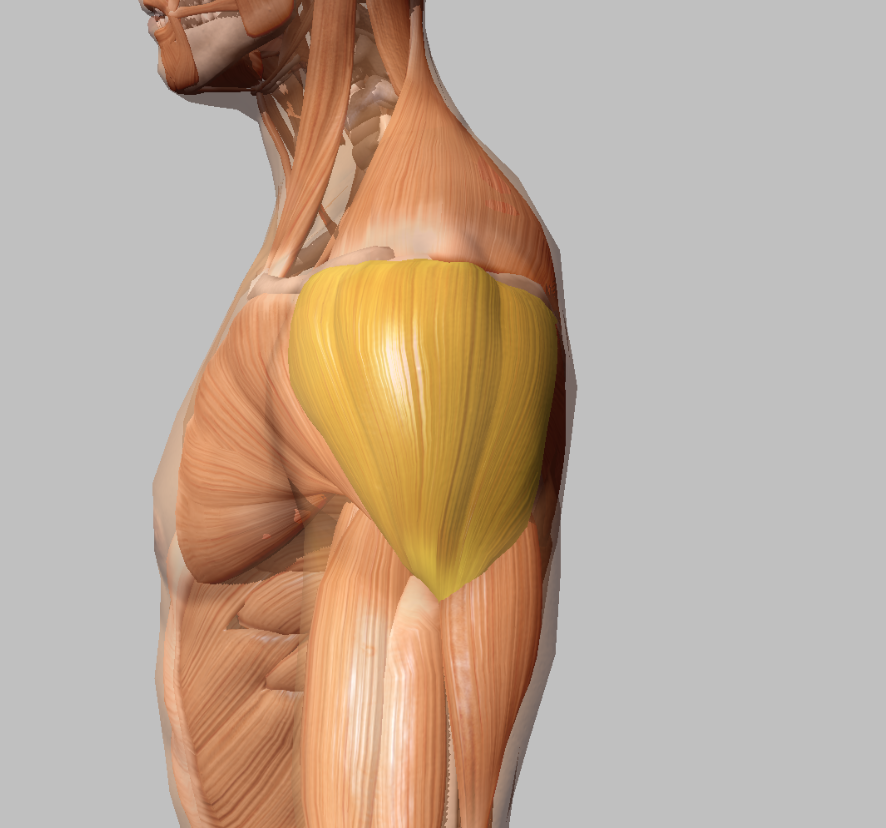
\includegraphics[width=\linewidth]{codelta.png}}


\newcommand{\omout}{ 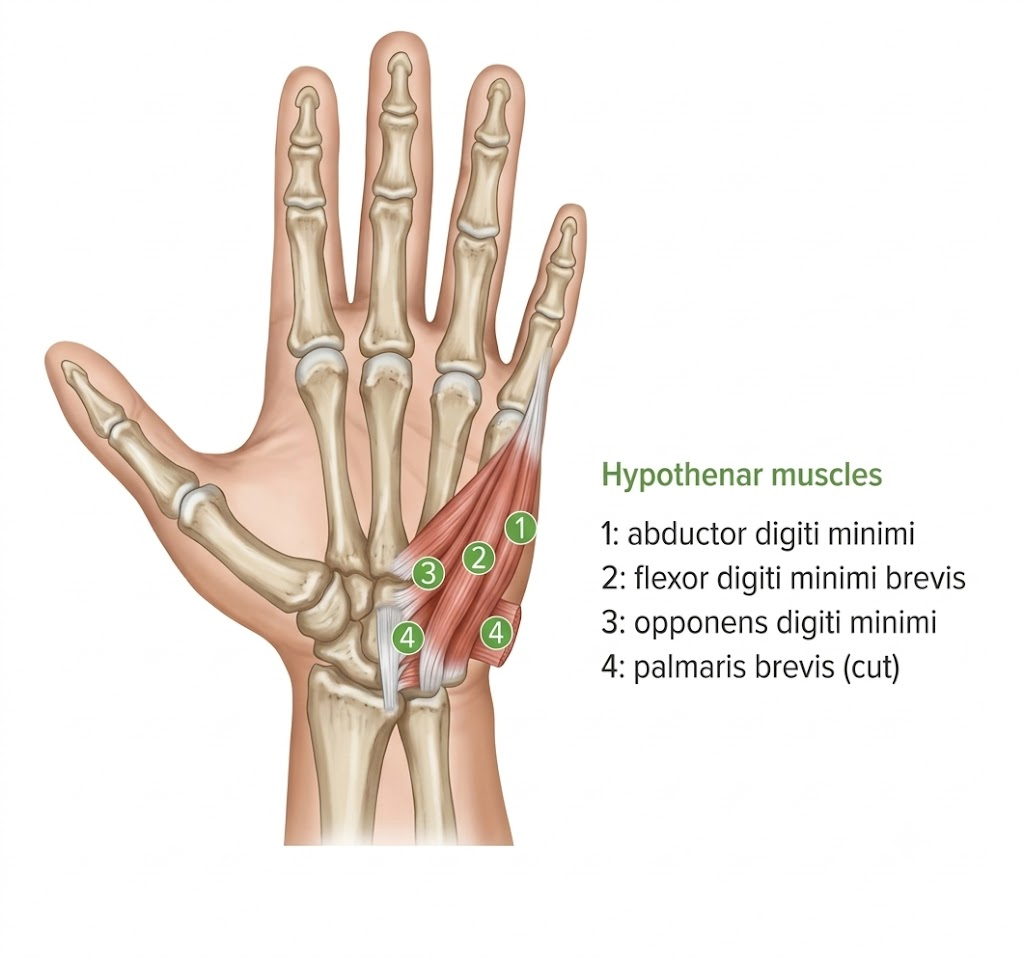
\includegraphics[width=1cm]{omout.png}}

\newcommand{\xoa}{\href{https://youtu.be/t8xlblzjSB0}{Xoa}}
\newcommand{\xat}{\href{https://youtu.be/5LxNXUudT0I}{Xát}}
\newcommand{\miet}{\href{https://youtu.be/C9047VbZbUE}{Miết}}
\newcommand{\phanhop}{\href{https://youtu.be/U7U3X2HWl14}{Phân hợp}}
\newcommand{\veo}{\href{https://youtu.be/Pooxu3bt3PU}{Véo}}
\newcommand{\vo}{\href{https://youtu.be/jX2Qz3dG_Fc}{Vỗ}}

\newcommand{\acday}{\href{https://youtu.be/BW-4i2ZW-V8}{Day}}
\newcommand{\dam}{\href{https://youtu.be/py1QDphCHxo}{Đấm}}
\newcommand{\chat}{\href{https://youtu.be/lzffl4TgL-I}{Chặt}}
\newcommand{\lan}{\href{https://youtu.be/2GyB6WE_xA4}{Lăn}}
\newcommand{\bop}{\href{https://youtu.be/ysqOetYi-L0}{Bóp}}
\newcommand{\von}{\href{}{Vờn}}

\newcommand{\cui}{\href{https://youtu.be/PqQY7ha7lAE}{Cúi}}
\newcommand{\ngua}{\href{https://youtu.be/aRl4YCO2omE}{Ngửa}}
\newcommand{\xoayphai}{\href{https://youtu.be/t8waFWkFmwU}{Xoay phải}}
\newcommand{\xoaytrai}{\href{https://youtu.be/urWJf_bhbUQ}{Xoay trái}}
\newcommand{\nhiengphai}{\href{https://youtu.be/noAQqTXWMBQ}{Nghiêng phải}}
\newcommand{\nhiengtrai}{\href{https://youtu.be/xn3b8cdrlU0}{Nghiêng trái}}
\newcommand{\xoayhonhop}{\href{https://youtu.be/S34xJ21dV3o}{Xoay hỗn hợp}}

\newcommand{\vandongco}{
Một tay để ở cằm, một tay để ở vùng chẩm. Hai tay vận động ngược chiều nhau một cách nhẹ nhàng, sau đó đột nhiên làm mạnh một cái sẽ phát ra tiếng kêu khục, rồi đổi chiều làm phía bên kia.

Khi vận động cổ cần chú ý bảo bệnh nhân để tự nhiên không chống đỡ (lên gân, rụt cổ lại). Nếu bệnh nhân có phản xạ chống đỡ thì vừa làm vừa nói chuyện với bệnh nhân, nếu thấy nhẹ dưới tay phải tranh thủ vận động cổ ngay.
}

\newcommand{\mbu}{\
Vận động cột sống tư thế nằm sấp bài ưỡn cột sống và thắt lưng cùng.\
Một tay đặt ở lưng dưới, tay còn lại ôm đầu gối (đùi dưới) bệnh nhân.\
Nâng đầu gối lên.\
}

\newcommand{\mfgd}{\
Vận động cột sống.\
Tư thế nằm ngửa.\
Một tay cầm cổ chân tay còn lại đặt lên đầu gối phía dưới.\
Đẩy đầu gối lên ngực kết hợp với xoay tròn.\
Sau đó hạ đầu gối về tư thế chuẩn bị.\
}

\newcommand{\mfvx}{\
Vận động cột sống.\
Tư thế nằm ngửa.\
Để bệnh nhân vào tư thế co chân vào bụng.\
Cánh tay dưới của một tay để ở đầu gối trên,
cánh tay dưới của tay còn lại để ở gần cổ chân.
Lòng bàn tay ôm xát mặt ngoài chân.
Đầu ngón tay có thể chạm vào đùi bệnh nhân.
Ghì xuống sao cho đốt thắt lưng cùng của bệnh nhân được giải phóng khỏi đệm.
Thực hiện xoay.
Chú ý hai đầu gối phải thẳng.\
}

\newcommand{\mfvgd}{\
Vận động cột sống.
Tư thế nằm ngửa.

Để bệnh nhân vào tư thế co chân vào bụng.\
Cánh tay dưới của một tay để ở đầu gối trên,
cánh tay dưới của tay còn lại để ở cạnh mông.

Nâng mông bệnh nhân lên\
}
